
\begin{figure*}%
\usetikzlibrary{arrows}
\usetikzlibrary{graphs,decorations.pathmorphing,decorations.markings}
\usetikzlibrary{calc}

\pgfmathsetmacro\weight{1/2}
\pgfmathsetmacro\third{1/3}
\pgfmathsetmacro\twothirds{2/3}

\tikzset{degil/.style={
          decoration={markings,
          mark= at position 0.5 with {
                 % \node[transform shape] (tempnode) {$\backslash$};
                \node[transform shape] (tempnode) {$/$};
                 }
             },
             postaction={decorate}
}
} 

%\usepackage{amsthm}
%\usepackage{amsmath} % assumes amsmath package installed
%\usepackage{amssymb}
%\newcommand \R   {\mathbb{R}}

\newcommand \qrq   {\quad\Rightarrow\quad}
\newcommand \qiq   {\quad\Iff\quad}


\newcommand \A   {\mathcal{A}}
\newcommand \OO   {\mathcal{O}}
\newcommand \B   {\mathcal{B}}
\newcommand \K   {\mathcal{K}}
%\newcommand \F   {\mathcal{F}}
\newcommand \Kinf{\mathcal{K_\infty}}
\newcommand \Linf  {\mathcal{L_\infty}}
\newcommand \KL  {\mathcal{KL}}
\newcommand \KKL  {\mathcal{KKL}}
\newcommand \LL  {\mathcal{L}}
\newcommand{\Knn}{\ensuremath{(\mathcal{K}_\infty\cup\{0\})^{n\times n}}}
\newcommand \PD   {\mathcal{P}}
%%%%%%%%%%%%% COPY TO QTIKZ   %%%%%%%%%%%%%%%%%%%%%%%%%%%%%%%%%

%\definecolor{GOcolor}{magenta}
\definecolor{GOcolor}{rgb}{0.858, 0.188, 0.478}
\definecolor{MPcolor}{rgb}{0, 0, 1}
\definecolor{HScolor}{rgb}{0.188, 0.858,  0.478}
%\definecolor{mypink2}{RGB}{219, 48, 122}

\small
\centering
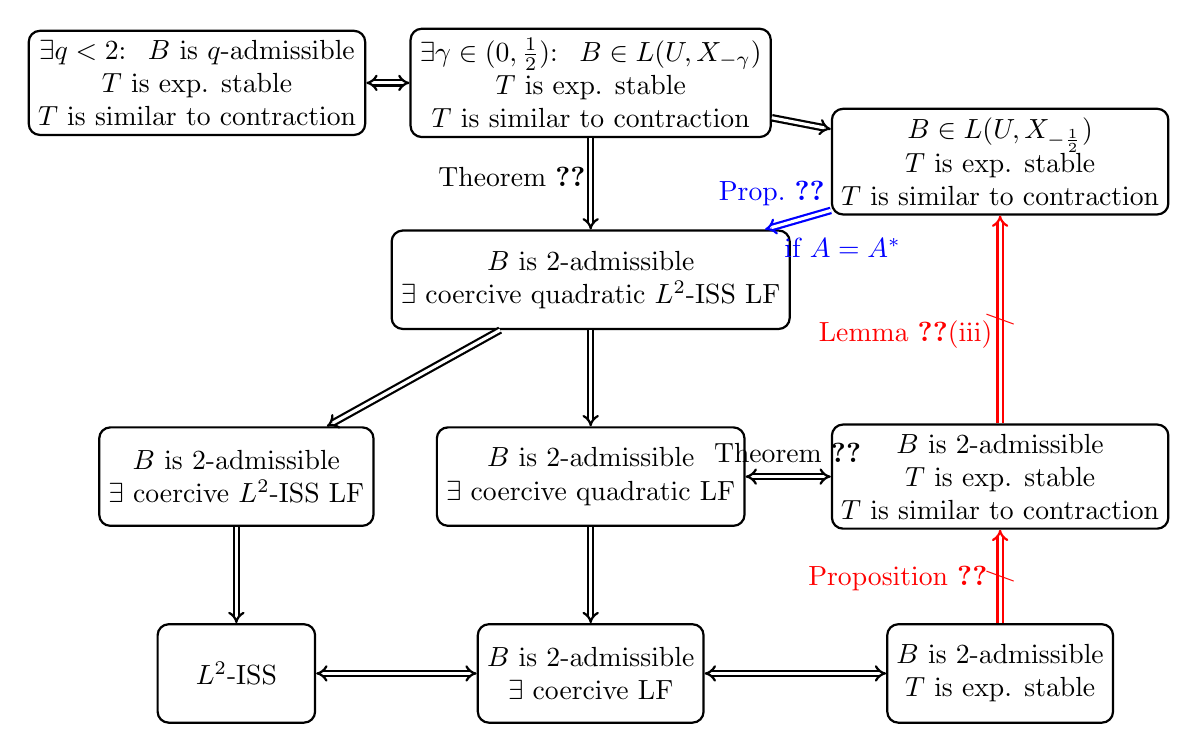
\begin{tikzpicture}[>=implies,thick, minimum height=1.25cm, minimum width=2cm]
%\node (Unif_Level) at (-4,5.5) {Uniform GAS level};
%\node (Nonunif_Level) at (-4.25, 2.5) {Non-uniform GAS level};

\node[draw, rounded corners, align=center] (AnSuff-2) at (-5.5,10) {$\exists q<2$: \ $B$ is $q$-admissible\\ $T$ is exp. stable\\ $T$ is similar to contraction};

\node[draw, rounded corners, align=center] (AnSuff) at (-0.5,10) {$\exists \gamma\in (0,\frac{1}{2})$: \ $B \in L(U,X_{-\gamma})$\\ $T$ is exp. stable\\ $T$ is similar to contraction};

\node[draw, rounded corners, align=center] (Self-AdSuff) at (4.7,9) {$B \in L(U,X_{-\frac{1}{2}})$\\ $T$ is exp. stable\\ $T$ is similar to contraction};

\node[draw, rounded corners, align=center] (quad-ISS-LF) at (-0.5,7.5) {$B$ is 2-admissible\\ $\exists$ coercive quadratic $L^2$-ISS LF};

\node[draw, rounded corners, align=center] (nonquad-ISS-LF) at (-5,5) {$B$ is 2-admissible\\ $\exists$ coercive $L^2$-ISS LF};

\node[draw, rounded corners, align=center] (quad-LF) at (-0.5,5) {$B$ is 2-admissible\\ $\exists$ coercive quadratic  LF};

\node[draw, rounded corners, align=center] (quad-LF-2) at (4.7,5) {$B$ is 2-admissible\\$T$ is exp. stable\\ $T$ is similar to contraction};


\node[draw, rounded corners, align=center] (L2-ISS) at (-5,2.5) {$L^2$-ISS};

\node[draw, rounded corners, align=center] (nonquad-LF) at (-0.5,2.5) {$B$ is 2-admissible\\ $\exists$ coercive LF};

\node[draw, rounded corners, align=center] (L2-ISS-crit) at (4.7,2.5) {$B$ is 2-admissible\\ $T$ is exp. stable};

\draw[thick,double equal sign distance,<->] (AnSuff) to (AnSuff-2);
\draw[thick,double equal sign distance,->] (AnSuff) to (Self-AdSuff);
\draw[thick,double equal sign distance,->] (AnSuff) to (quad-ISS-LF);
\draw[color = blue, thick,double equal sign distance,->] (Self-AdSuff) to (quad-ISS-LF);
\node[color=blue] (Self-Ad) at (2.7,7.9) {if $A=A^*$};
\node (Self-Ad) at (2,5.3) {Theorem~\ref{thm:Quad-coercive-nonanalytic-1}};
\node[color=blue] (Self-Ad) at (1.8,8.6) {Prop.~\ref{prop:Coercive-LF-Self-adjoint}};
\node (Self-Ad) at (-1.5,8.8) {Theorem~\ref{thm:Coercive-LFs-for-admissible-operators}};
%\node (Self-Ad) at (5.7,9.9) {\todo{Counterexample for the converse implication?}};
%\node (Self-Ad) at (-2.7,10.3) {\todo{}};
%\draw[thick,double equal sign distance,->] (quad-ISS-LF) to (L2-ISS);
\draw[thick,double equal sign distance,->] (quad-ISS-LF) to (quad-LF);
\draw[thick,double equal sign distance,->] (quad-ISS-LF) to (nonquad-ISS-LF);
\draw[thick,double equal sign distance,<->] (quad-LF-2) to (quad-LF);

\draw[thick,double equal sign distance,->] (nonquad-ISS-LF) to (L2-ISS);

\draw[thick,double equal sign distance,->] (quad-LF) to (nonquad-LF);
\draw[thick,double equal sign distance,<->] (L2-ISS-crit) to (nonquad-LF);
\draw[thick,double equal sign distance,<->] (nonquad-LF) to (L2-ISS);

\draw[thick,double equal sign distance,->,degil,red] (L2-ISS-crit) to (quad-LF-2);
\draw[thick,double equal sign distance,->,degil,red] (quad-LF-2) to (Self-AdSuff);
\node[color=red] (TuW09) at (3.5,6.8) {Lemma~\ref{lem:Sufficient-condition-for-admissibility}(iii)};

\node[color=red] (TuW09) at (3.4,3.7) {Proposition~\ref{prop1}};

\end{tikzpicture}
\caption{$L^2$-ISS, $L^2$-ISS Lyapunov functions, and admissibility for analytic linear systems}%
\label{fig:Overview-of-results}%
\end{figure*}
